\documentclass[]{scrartcl}
\title{Vorlesung Analysis II}
\usepackage{amsmath,amssymb,amsfonts}
\usepackage{stmaryrd}
\usepackage{mathtools}
\usepackage{latexsym}
\usepackage{graphicx}
\usepackage{tikz}
\usepackage{xcolor}
\usepackage{soul}
\usepackage{hyperref}
\usepackage{tipa}
\usepackage[normalem]{ulem}
\usepackage[dvipsnames]{xcolor}
\hypersetup{
	colorlinks=true,
	linkcolor=blue,
	filecolor=magenta,      
	urlcolor=cyan,
	pdftitle={Overleaf Example},
	pdfpagemode=FullScreen,
}
\newcommand{\redcircle}[1]{%
	\tikz[baseline=(char.base)]{
		\node[shape=circle, draw=red, text=red, thick, inner sep=1pt] (char) 
		{\textbf{#1}};
	}%
}
\newcommand{\bluecircle}[1]{%
	\tikz[baseline=(char.base)]{
		\node[shape=circle, draw=blue, text=blue, thick, inner sep=1pt] (char) 
		{\textbf{#1}};
	}%
}
\newcommand{\blackcircle}[1]{%
	\tikz[baseline=(char.base)]{
		\node[shape=circle, draw=black, text=black, thick, inner sep=1pt] (char) 
		{\textbf{#1}};
	}%
}
\setul{1pt}{3pt} % Linienhöhe und Abstand zum Text (optional anpassbar)

\setlength{\topmargin}{-.5in} \setlength{\textheight}{9.25in}
\setlength{\oddsidemargin}{0in} \setlength{\textwidth}{6.8in}
\setlength{\parindent}{0pt}

\begin{document}
	\textbf{\underline{Teil 2: Topologische Grundbegriffe in metrischen Räumen}}\\
	\\
	\textbf{\underline{an12:Konvergenz und Kompaktheit}}\\
	\\
	\textbf{\underline{\underline{Stichworte:} Vollständigkeit, allg. Banach-Fixpunktsatz, Kompaktheit, Heine-Borel}}\\
	\\
	\underline{Literatur:} \setulcolor{blue} \ul{[Forster], Kapitel 3}\\
	\\
	\textbf{12.1. \underline{Einleitung:}} $\mathbb{R}^n$ ist als metrischer Raum vollständig. Wir zeigen, dass abgeschlossene Teilmengen eines vollständigen metrischen Raums wieder Vollständig sind, was einen neuen Blick auf den Banachschen Fixpunktsatz wirft.
	Weiter werden wir zum Kompaktheitsbegriff geführt, und wir zeigen den Satz von Heine-Borel, welcher besagt, dass die (überdeckungs-)kompakten Teilmengen im metrischen Raum $\mathbb{R}^n$ genau die sin,  die beschränkt und abgeschlossen sind.\\
	\\
	\textbf{12.2 \underline{Motivation:}} Sei $\o \neq M \subseteq (R,\delta)$, dann ist \setulcolor{green} \ul{$(M,\delta_{\neg MxM})$ auch metrischer Raum.}\\
	Für $a \in M$ ist dann eine Kugel in M um a:\\
	\setulcolor{yellow} \ul{$B_{a,n}^\epsilon$}:=$\{x\in\mathbb{R};\delta(x,a)<\epsilon\}\cap M = B_{a,R}^\epsilon\cap M.$\\
	\begin{figure}[h]
		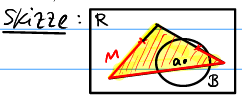
\includegraphics[width=7 cm,height=3cm]{bsp kap 12.2}
	\end{figure}\\
	\underline{Beobachtung:} $B_{a,n}^\epsilon$ offen in M, i.a. aber nicht in R.\\
	\\
	\textbf{12.3 \underline{Bezeichnung:}} in M \setulcolor{red} \ul{relativ offen} :$\Leftrightarrow$ offen in M\\
	in M \ul{relativ abgeschlossen}:$\Leftrightarrow$ abg. in M\\
	\\
	\textbf{12.4} Es gibt: \\
	$M\supseteq U$ \setulcolor{green} \ul{odden in M} $\Leftrightarrow$ \ul{$O \in \mathcal{O}(R):U=O\cap M$},\\
	$M\supseteq U$ \ul{abg. in M} $\Leftrightarrow$ \ul{$\exists A \in \mathcal{A} (R):A\cap M$}.\\
	\\
	\textbf{12.5. \underline{Bem.:}} Sei $a\in M \subseteq R.$\\
	(1) \ul{$a\in \dot{M}$} $\Leftrightarrow \forall k \in \mathbb{N}$ \ul{$\exists x_k \in M \backslash\{a\}:x_k\rightarrow a$},\\
	(2) \ul{$a \in \overline{M}$} $\Leftrightarrow \forall k \in \mathbb{N}$ \ul{$\exists x_k \in M: x_k \rightarrow a$}.\\
	\underline{Bew.:} Zu (1): "$\Rightarrow$: $a \in \dot{M} \Rightarrow \exists x_k \in (U_a^{\frac{1}{k}}\backslash\{a\})\cap M \Rightarrow x_k\rightarrow a.$\\
	"$\Leftrightarrow$" vgl. Def. HP in \setulcolor{blue}\ul{11.14}: In jeder Umgebung von $x_k$ lieden $\infty$ viele Folgenglieder $\Rightarrow$ a ist HP.\\
	Zu (2): $\overline{M} = M\cup \dot{M}$ aus \ul{(1)}.\\
	\\
	\textbf{12.6. \underline{Satz:}}(R.S) \setulcolor{green}\ul{vollständig, $M\subseteq R$}.\\
	\underline{Beh.:} \ul{M vollständig $\Leftrightarrow$ M Abgeschlossen}.\\
	\underline{Bew.:}"$\Rightarrow$": Zeige $M=\overline{M}$ oder: $a\in\overline{M} \xRightarrow{12.3(2)} \exists(x_k)\subseteq M, x_k \rightarrow a \Rightarrow (x_k)$ ist CF\\
	$\Rightarrow$a = $lim x_k \in M,$ da M vollständig nach Vor.\\
	"$\Leftarrow$":$(x_k)$ CF in M $\Rightarrow (x_k)$ CF in $R\Rightarrow \exists a \in R: x_k \rightarrow a \Rightarrow a\in \overline{M}=M.$\\
	\strut\hfill$\square$\\
	Wir erhalten weiter die allgemeine Version der Banachschen Fixpunktsatzes in \underline{vollständigen} metrischen Räumen wie folgt.\\
	\\
	\textbf{12.7. \setulcolor{red}\ul{Banachscher Fixpunktsatz(allg. Version):}}\\
	\underline{Vor.:} $(R,\delta)$ \setulcolor{green}\ul{vollständiger metrischer} Raum, f: \ul{$R\rightarrow R$ Kontraktion} mit Kontraktionsfaktor $p\in[0,1[.$\\
	\underline{Beh.:} \\
	a) \ul{$\exists!$ Fixpunkt a von f}.\\
	b) Setze \ul{$x_0 \in R$} beliebig und \ul{$x_{k+1} := f(x_k)$} für alle k $\geq$0.\\
	Dann: \ul{$\delta(x_k,a) \leq \frac{p^k}{1-p}\delta(x_1,x_0)$}, d.h. insb. \ul{$\lim_{k\rightarrow\infty}x_k=a$}.\\
	\\
	\underline{Bew.:} Wie in \setulcolor{blue} \ul{8.6} zeigt mann, dass ($x_k$) eine CF ist.\\
	Da R vollständig, ex. $a=\lim_{k\rightarrow\infty}x_k \in R.$ wie dort zeigt man f(a)=a.\\
	\strut\hfill$\square$\\
	\textbf{12.8 \underline{Bem.:}} Da der frühere Fixpunktsatz für Kontraktionen auf $U \subseteq \mathbb{R}^n$ formuliert ist, wo U abg. \sout{und beschr. ist(also Kompakt nach kap 12.11)} und somit vollständig nach \ul{12.6}, und \ul{$\redcircle{Ü}$ Bl. 2A2.2}\setulcolor{green}(\ul{$\mathbb{R}^n$ ist vollständig}), folgt die alte version \setulcolor{blue} \ul{8.6} auch aus \ul{12.7}.\\
	\\
	Für bestimmte Anwendungen(z.b Existenz von Extrema auf bestimmten Teilmengen des $\mathbb{R}^n$) reicht die Abgeschlossenheit oft nicht aus, wir benötigen dafür einen stärkeren Begriff wie folgt.\\
	\\
	\textbf{12.9. \underline{Def.:}} $M\subseteq R$ heißt \setulcolor{red}\ul{Kompakt} (auch:"\ul{überdeckungskompakt}"), falls gilt:\setulcolor{blue} \ul{Jede offene Überdeckung von M hat eine endliche teilüberdeckung, *} d.h. $M\subseteq \bigcup_{i\in I}=O_i$ mit $O_i\infty \mathcal{O}(R)\Rightarrow \exists$ endlich viele $O_{i_1},...,O_{i_k}$, die $i_1,...,i_k  \in I: M\subseteq \bigcup_{i=1}^kO_{i_1}=o\cup ...\cup O_{i_k}.$\\
	\\
	\textbf{12.10. \underline{Bem.:}} Die Aussage \bluecircle{*} wird manchmal missverstanden in der Form "Nur endlich viele Überdeckungsmengen $O_i$ überdecken M nur zum Teil" o.ä. gemeint ist aber, dass stets bereits endlich vile Überdeckungsmengen zur Kompletten Überdeckung der Menge M ausreichen ("Teil" bezieht sich auf die Indexmenge I).\\
	\\
	\textbf{12.11. \underline{Bsp.:}} $M=[0,1]\subseteq \mathbb{R}^1$, für $t\in[0,1]$ bilden mit bel. $\epsilon_t\textgreater0$ die "Kugeln" $B_t^{\epsilon_t}=]t-\epsilon_t, t+\epsilon_t[$ bereits eine Überdeckung von $[0,1]$, denn $[0,1]\subseteq \bigcup_{t\in[0,1]}B_{t}^{\epsilon_t}.$\\
	Nun ist $[0,1]$ Kompakt laut \ul{12.11}, also $\exists t_1,...,t_n\in[0,1]\exists \epsilon_1,...,\epsilon_n\textgreater 0:[0,1]\subseteq\bigcup_{j=1}^nB_{t_j}^{\epsilon_j}.$[anschaulich klar]
	\begin{figure}[h]  
		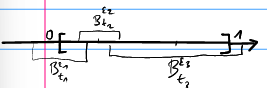
\includegraphics[width=5cm,height=2cm]{bsp kap 12.11}
	\end{figure}\\
	Eine auf M stetige Funktion $f:M\rightarrow\mathbb{R}$ nimmt ihr mMinimum und Maximum an, vgl. Satz von Minimum/Maximum An9.30.\\
	Als Anwendung ddes Zwischenwertsatzes erhält man, dass $f(u)\subseteq\mathbb{R}$ ein abg. IV ist.\\
	\\
	\textbf{12.12. \underline{Bsp.:}} $M=]0,1] \subseteq \mathbb{R}^1$ ist nicht Kompakt, denn in der Überdeckung $]0,1] \subseteq \bigcup_{n\in\mathbb{N}}B_{1/n}^{1/2n}$ kann keine endliche Teilüberdeckung ausgewähl werden, die zur Überdeckung von ]0,1] bereits ausreichen würde.\\
	Hier gibt es eine M stetige Funktion $f:M\rightarrow\mathbb{R},$ die kein Maximum annimmt, z.b. $f:M\rightarrow\mathbb{R}, f(x)=\frac{1}{x}$.\\
	\\
	\textbf{12.13. \underline{Bsp.:}} Die Menge M=$[0,\infty[\subseteq\mathbb{R}, f(x)=\frac{1}{x}$.\\
	\\
	\textbf{12.13. \underline{Bsp.:}} Die Menge $M=[0,\infty[\subseteq\mathbb{R}^1$ ist nicht Kompakt, wie die Überdeckung $[0,\infty[\subseteq \bigcup_{n\geq 1}N_n^{1.1}$ zeigt. Die Funktion $f:M\rightarrow\mathbb{R}, f(x)=x$, nimmt kein Maximum an.\\
	\\
	Im $\mathbb{R}^n$ lässt sich Kompaktheit einfach topologisch beschreiben wie folgt.\\
	\textbf{12.14\setulcolor{red} \ul{Satz (von Heine-Borel):}}\\
	Sei \setulcolor{green}\ul{$M\subseteq\mathbb{R}^n$} und $\mathbb{R}^n$ mit einer Metrik versehen, die assoziert von einer Norm ist ($\OE$ also $||\cdot=||\cdot||_infty$).\\
	Dann sind \ul{äquivalent}: \\
	(a)\ul{M ist Kompakt},\\
	(b)\ul{M ist Folgenkompakt},\\
	d.h. jede Folge in M hat eine (in M) Konvergent Teilfolge,\\
	(c)\ul{M ist beschränkt und abgeschlossen}.\\
	\underline{Bew:} (\setulcolor{orange}\ul{Ringschluss $(a)\Rightarrow(c)\Rightarrow(b)\Rightarrow(a)$}):\\
	\underline{zu $(a)\Rightarrow(c)$}: Sei M Kompakt. \\
	(i:) Mit $M\subseteq \mathbb{R}^n=\bigcup_{m\in\mathbb{N}}B_0^m$ Folgt dann:\\
	$\exists m_0\in\mathbb{N}:M\subseteq\bigcup_{m\leq m_0}B_0^m=B_0^{m_0}\Rightarrow||M||_\infty \leq m_0,$ also ist M beschränkt.\\
	(ii): Sei $x \in \mathcal{C}M=\mathbb{R}^n\backslash M$ fest, wähle \setulcolor{orange}\ul{$U^{(y)}\in \mathcal{U}_x$} und \ul{$V^{y}\in \mathcal{U}_y$} offen für alle $y\in M$ so, dass $U^{(y)}\cap V^{y}=\o.$ \ul{($\mathbb{R}^n$ ist hausdorffsch)}\\
	Also ist $M\subseteq \bigcup_{y\in M} V^{(y)}$ \ul{offenen Überdeckung}.\\
	\begin{figure}[h]  
		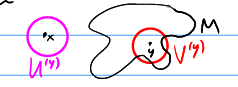
\includegraphics[width=5cm,height=2cm]{bsp kap 12.14}
	\end{figure}\\
	Da M Kompakt ist, ex. $V^{(y_1)},...,V^{(y_n)}$ mit $M\subseteq \bigcup_{j=1}^n V^{(y_j)}$.\\
	Setze $\mathcal{U}_x \ni$ \ul{$U:\bigcap_{j=1^n U^{(y_j)}}$}, dies ist eine offene Umgebung von x.\\
	damit ist dann \ul{$U \cap M = \o$}, d.h. $ U\subseteq\mathcal{C}M\Rightarrow\mathcal{C}M$ offen $\Rightarrow M$ abgeschlossen.\\
	Zu $(c)\Rightarrow(a): (i):z.z.: M$ abg., also nach \setulcolor{blue} \ul{12.6} \underline{vollständig}.\\
	denn: $z\in\overline{M} \Rightarrow \exists x_k \rightarrow z$(Kgz.),($x_k$)$\subseteq M$ und ($x_k$) hat \ul{nach (b)} eine in M Konvergente Teilfolge (mit demselben GW)$\Rightarrow x_k\rightarrow z \in M.$\\
	(ii) z.z.: M ist \setulcolor{red}\ul{total beschränkt}, d.h. $\forall\epsilon\textgreater 0 \forall M_0 \subseteq M, M_0$ endl. $\exists x \in M\backslash \bigcup_{a\in M_0}B_a^\epsilon.\\
	\textopencorner$ Ann.: M wäre nicht total beschränkt, d.h. $\exists \epsilon \textgreater 0 \forall M_0 \subseteq M, M_0$ \underline{endl.:} $M \subseteq\bigcup_{a\in M_0}B_a^\epsilon.$\\
	Wähle $x_1\in M$ und $x_k$ induktiv für $k\geq2: x_k \in M\backslash\bigcup_{j=1}^{k-1} B_{x_j}^\epsilon.$\\
	Dann gilt: $(x_k)\subseteq M$ mit $\delta(x_i,x_j)\geq \epsilon$ für alle $i,j\in \mathbb{N},$ d.h. ist keine CF und auch keine Teilfolge, d.h. $(x_k)$ hat keine Konvergente Teilfolge im $\lightning$ \setulcolor{blue} \ul{zu (b)}.\textcorner\\
	Benötigen (i) und (ii) für Schritt (iii) des (eigentlichen) Beweises:\\
	(iii)z.z.: M ist Kompakt (indirekt):\\
	Für k$\subseteq$ R nicht Kompakt gilt: $ \exists \mathcal{O}_1\subseteq \mathcal{O}: K\subseteq \bigcup_{O \in \mathcal{O}_1}O \Rightarrow \forall \mathcal{O}_2\subseteq \mathcal{O}_1$ endl.: $ K\nsubseteq \bigcup_{O \in \mathcal{O}_2}O.$\\
	Sei dies so für M, dazu $\mathcal{O}_1$ geg. mit $M\subseteq \bigcup_{O \in \mathcal{O}_1}O.$\\
	$\bullet$ Zu $\epsilon=2^{-1}$ gilt nach (ii): $\exists M_1 \subseteq M$ endlich: $ M\subseteq \bigcup_{a\in M_1} B_a^{2^{-1}} \rightarrow \forall\mathcal{O}_2\subseteq\mathcal{O}_1$ endlich: $M\nsubseteq \bigcup{O\in\mathcal{O}_2}O$\\
	$\Rightarrow\exists x_1\in M_1\forall \mathcal{O}_2 \subseteq\mathcal{O}_1$ endlich: $M\cap B_{x_1}^{2^{-1}}\nsubseteq \bigcup_{O \in \mathcal{O}_2}O,$ d.h. $M\cap B_{x_1}^{2^{-1}}$ nickt Kp.(kompakt)\\
	\textopencorner sonst: $\forall a\in M_1: B_a^{2^{-1}} \cap M \subseteq \bigcup_{O \in \mathcal{O}_2}O$ für ein $\mathcal{O}_2 \subseteq \mathcal{O}_1$ endlich $\rightarrow$ endlich viele $O\in\mathcal{O}_1$ würden $M=\bigcup_{a\in M_1}B_a^{2^{-1}}\cap M$ Überdecken $\lightning$\textcorner\\
	$\bullet$ Zu $\epsilon = 2^{-\textcolor{red}{2}}$ gilt \setulcolor{blue} \ul{nach (ii)}: $\exists M_{\textcolor{red}{2}}\subseteq M$ endlich: $M \subseteq \bigcup_{O \in \mathcal{O}_{\textcolor{red}{2}}} B_a^{2^{-\textcolor{red}{2}}}$\textcolor{red}{, d.h. $M \cap B_x{x_1}^{2^{-1}}\subseteq \bigcup_{O \in \mathcal{O}_2} B_a^{21{-2}}.$}\\
	$\xRightarrow{ebenso}\exists x_{\textcolor{red}{2}}\in M_{\textcolor{red}{2}}\forall \mathcal{O}_2\subseteq\mathcal{O}_1$ endlich: $M\cap B_{x_1}^{2^{-1}}$\textcolor{red}{$\cap B_{x_2^{2{-2}}}$} $\nsubseteq \bigcup_{O \in \mathcal{O}_2}O, d.h. M\cap b_{x_1^{2^{-1}}}$\textcolor{red}{$\cap B_{x_2^{2{-2}}}$} nicht Kp.\\
	$\bullet$ Zu $\epsilon = 2^{-\textcolor{red}{k}}$ gilt \ul{nach (ii)}: $\exists M_{\textcolor{red}{k}} \subseteq M$ endlich: $M\subseteq \bigcup_{a\in M_{\textcolor{red}{k}}}B_a^{2^{-\textcolor{red}{k}}}$\textcolor{red}{, d.h. $M\cap B_{x_1}^{2^{-k+1}}\subseteq \bigcup_{a\in M_{\textcolor{red}{k}}} B_a^{2^{-k}}.$}\\
	$\xRightarrow{ebenso}\exists x_{\textcolor{red}{k}}\in M_\{\textcolor{red}{k}\} \forall \mathcal{O}_2\subseteq\mathcal{O}_1$ endlich: $M\cap $\textcolor{red}{$\underbrace{B_{x_1}^{2^{-1}} ßcup...\cup B_{x_k}^{2^{-k}}}_{=:B_k}$} $\nsubseteq \bigcup_{O \in \mathcal{O}_2}O,$\\
	d.h. $M\cap B_{x_1}^{2^{-1}}$\textcolor{red}{$\cap...\cap B_{x_k}^{2^{-k}}=M\cap B_k$} nicht Kp.\\
	Es ist $B_k \neq \emptyset,$ sonst wäre $\emptyset=M\cap B_k \nsubseteq \bigcup_{O \in \mathcal{O}_2}O.$ Somit $\exists v_k \in B_k$ für $k\geq2.$\\
	Dann gilt: $\delta(x_{k-1},x_{k})\leq \delta(x_{k-1},v_k)+\delta(v_k,x_k)\leq \frac{1}{2^{k-1}}+\frac{1}{2^k}\textless \frac{1}{2^{k-2}}\Rightarrow(x_k)$ ist eine CF.\\
	\ul{Nach (i)} gilt: $x_k\rightarrow x_0 \in M.$\\
	sei $B_0$ eine Kugel um $x_0$.\\
	Dann gibt es ein k so, dass $B_k \subseteq B_0.$ Wählt man insbesondere $B_0\subseteq O\in \mathcal{O}_1.$\\
	\begin{figure}[h]  
		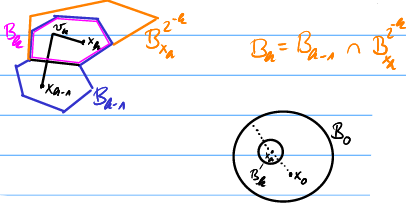
\includegraphics[width=5cm,height=2cm]{bsp kap 12.14.2}
	\end{figure}\\
	\textopencorner denn $x_0\in M$ wird von einem $O\in \mathcal{O}_1$ offen überdeckt und $x_0\in B_0,$ für $B_0$ klein\textcorner\\
	so folgt $B_k \subseteq B_0\subseteq O \in \mathcal{O}_1,$ also $M\cap B_k \subseteq = \in \mathcal{O}_1.$\\
	Setze $\mathcal{O}_2=\{O\}\subseteq \mathcal{O}_1$ (ist endlich), also $M\cap B_k\subseteq \bigcup_{O \in \mathcal{O}_2}O, \lightning$ gegen obige Konstruktion.\\
	\strut\hfill$\square$\\
	\textbf{12.15. \underline{Bem.:}} Ein \setulcolor{green}\ul{metrische Raum} ist genau denn \ul{Kompakt}, wenn er \ul{vollständig und total beschränkt} ist.\\
	Der vorige Beweis kann dahingehend angepasst werden.\\
	\\
	Die folgende Aussage ist ein "Schachtelungsprinzip" für Kompakte Mengen.\\
	\textbf{12.16. \underline{Satz:}} Vor.: $(R,\delta)$ \ul{metrischer Raum, $\o\neq A_k$}$\subseteq R, k\in \mathbb{N},$ \ul{$A_k$ kompakt},\\
	$\forall k \in \mathbb{N}:$ \ul{$A_k\supseteq A_{k+1}$}.\\
	\underline{Beh.:} \ul{$\bigcap_{k=1}^\infty A_k\neq \o$.}\\
	\underline{Bew.:} Ann.: $\bigcap_{k=1}^\infty A_k=\o \Rightarrow \mathcal{C}(\bigcap_{k=1}^\infty A_k)=R$\\
	$\Rightarrow A_1 \subseteq R = \bigcup_{k=1}^\infty \underbrace{\mathcal{C}A_k}_{\text{offen}}\xRightarrow{A_1 Kp.} \exists k_0: A_{k_0}\subseteq A_1\subseteq \bigcup_{k=1}^{k_0}\mathcal{C} A_k=\mathcal{C}A_{k_0}\\
	\Rightarrow A_{k_0} = \o, \lightning.$\\
	\strut\hfill$\square$\\
	\textbf{12.17. \underline{Bsp.:}} $\bigcap_{n\in\mathbb{N}}[-\frac{1}{n},\frac{1}{n}]=\{0\}, \bigcap_{n\in\mathbb{N}}\{x\in\mathbb{R}_{\textgreater0};|x^2-2|\leq\frac{1}{n}\}=\{\sqrt{2}\},$\\
	aber $\bigcap_{n\in\mathbb{N}}\{x\in\mathbb{Q}_{\textgreater0};|x^2-2|\leq\frac{1}{n}\}=\o$ \redcircle{Ü}\textcolor{red}{warum?}
	
	
	
	
	
	
	
	
	
	
	
	
	
	
	
	
	
	
\end{document} 
